\documentclass[11pt,letterpaper,boxed]{pset}

\usepackage[margin=0.75in]{geometry}
\usepackage{ulem}

\name{Name: \rule{2.5cm}{0.15mm}}
\assignment{Box \# \rule{1.5cm}{0.15mm}}
\class{MATH060 HW7}

\begin{document}

    \problemlist{MATH060 HW7}
    \begin{center}
    	4.2: 6, 12, 28, 29 \\
    	4.3: 24, 26
    \end{center}
    
    \begin{problem} [4.2.6]
    	Identify and determine the nature of the critical points of the given function.
    
    	\[ f(x,y) = y^4 - 2xy^2+x^3 -x \]
    
    \end{problem}
    \newpage
    
    
    \begin{problem} [4.2.12]
    	Identify and determine the nature of the critical points of the given function.
    
    	\[f(x,y) = e^{-x}(x^2+3y^2)\]
    
    \end{problem}
    \newpage
    
    
    \begin{problem} [4.2.28]
    	Show that the largest rectangular box having a fixed surface area must be a cube.
    
    \end{problem}
    \newpage
    
    
    
    \begin{problem} [4.2.29]
    	What point on the plane $3x − 4y − z = 24$ is closest to the origin?
    
    \end{problem}
    \newpage
    
    
    \begin{problem} [4.3.24]
    	You are sending a birthday present to your calculus instructor.Fly-By-Night Delivery Service insists that any package it ships be such that the sum of the length plus the girth be at most 108 in. (The girth is the perimeter of the cross section perpendicular to the length axis\textemdash see Figure 1.) What are the dimensions of the largest present you can send?
    
    
    \end{problem}
    
    \begin{figure}[h!]
        \begin{center}
            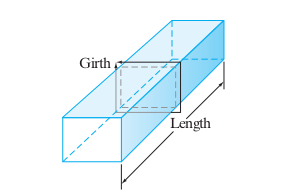
\includegraphics[width=60mm]{box.png}
        \end{center}
    \end{figure}
    
    \newpage
    
    
    \begin{problem} [4.3.24]
    	An industrious farmer is designing a silo to hold her $900\pi \textrm{ft}^3$ supply of grain. The silo is to be cylindrical in shape with a hemispherical roof. (See the Figure.) Suppose that it costs five times as much (per square foot of sheet metal used) to fashion the roof of the silo as it does to make the circular floor and twice as much to make the cylindrical walls as the floor. If you were to act as consultant for this project, what dimensions would you recommend so that the total cost would be a minimum? On what do you base your recommendation? (Assume that the entire silo can be filled with grain.)
    
    \end{problem}
    
    \begin{figure}[h!]
        \begin{center}
            
\includegraphics[width=20mm]{silo.png}
        \end{center}
    \end{figure}

    \newpage
    
\end{document}